\documentclass{article}
\usepackage{graphicx}
\usepackage{caption}
\usepackage{subcaption}
\graphicspath{{./figs/}}{}
\usepackage{listings}
\title{
HLS-Assignment 5A
}
\begin{document}
\maketitle
\hfill \textbf{Sampath Govardhan} \\
\null \hfill \textbf{FWC22071}\\

\section{Problem Statement}
\begin{lstlisting}
Implement a DUT that accesses 8 elements from BRAM (the BRAM should be 
contained within the DUT, you can choose to populate the BRAM in any way
you like) and gives out all 8 values as HLS streaming output in a single 
bundle in a single clock cycle. The starting index will be an input to the 
DUT and it will be a multiple of 8.

The way to access these 8 elements are as follows:

1. 8 consecutive elements are to be chosen and these elements will make up 
a bundle.
2. Every 8th element is to be chosen and 8 such elements will make up a bundle.


\end{lstlisting}
\vspace{10cm}


\section{Design Code}
\textbf{5.1}
\begin{lstlisting}
#include "hls_stream.h"
#include "ap_int.h"
//#include "ap_axi_sdata.h"

typedef ap_uint<8> in;

struct bundle{
in data[8];
};


void a5a(int index,hls::stream<bundle> &output){

in bram[64]={0,1,2,3,4,5,6,7,8,9,10,11,12,13,14,15,16,17,18,19,20,21,
22,23,24,25,26,27,28,29,30,31,32,33,34,35,36,37,38,39,40,41,42,43,44,45,46,47,48,
49,50,51,52,53,54,55,56,57,58,59,60,61,62,63};

#pragma HLS RESOURCE variable=bram core=RAM_1P_BRAM
#pragma HLS ARRAY_PARTITION variable=bram cyclic factor=8 dim=1

bundle out={bram[index],bram[index+1],bram[index+2],bram[index+3],bram[index+4],
		bram[index+5],bram[index+6],bram[index+7]};
output.write(out);
}


\end{lstlisting}
\vspace{10cm}
\textbf{5.2}
\begin{lstlisting}

#include "hls_stream.h"
#include "ap_int.h"
//#include "ap_axi_sdata.h"

typedef ap_uint<8> in;

struct bundle{
in data[8];
};


void a5a(int index,hls::stream<bundle> &output){

in bram[64]={0,1,2,3,4,5,6,7,8,9,10,11,12,13,14,15,16,17,18,19,20,21,
22,23,24,25,26,27,28,29,30,31,32,33,34,35,36,37,38,39,40,41,42,43,44,45,46,47,48,
49,50,51,52,53,54,55,56,57,58,59,60,61,62,63};

#pragma HLS RESOURCE variable=bram core=RAM_1P_BRAM
#pragma HLS ARRAY_PARTITION variable=bram block factor=8 dim=1

bundle out={bram[index],bram[index+8],bram[index+16],bram[index+24],bram[index+32],
		bram[index+40],bram[index+48],bram[index+56]};
output.write(out);
}

\end{lstlisting}
\vspace{10cm}


\section{Test Bench Code}
\textbf{5.1 and 5.2}
\begin{lstlisting}

#include <fstream>
#include "hls_stream.h"
#include "ap_int.h"
using namespace std;

typedef ap_uint<8> in;

struct bundle{
in data[8];
};

void a5a(int index,hls::stream<bundle> &output);

int main(){
hls::stream<bundle> out_stream;
int index,a,b,c,d,e,f,g,h;
bool fail=0;

ifstream ref("in.dat");
ofstream res("out.dat");

for (int i=0;i<8;i++){
	ref>>index>>a>>b>>c>>d>>e>>f>>g>>h;
a5a(index,out_stream);
bundle out=out_stream.read();
for (int j=0;j<8;j++){
res<<out.data[j]<<" ";
}
if (out.data[0]==a && out.data[1]==b && out.data[2]==c &&
out.data[3]==d && out.data[4]==e && out.data[5]==f && out.data[6]==g &&
out.data[7]==h ){
res<<"Pass"<<endl;
}
else{
res<<"Fail"<<endl;
fail=1;
}
}
ref.close();
res.close();
if (fail==0){
cout<<"ALL THE TEST CASES ARE PASSED!"<<endl;
}
else{
cout<<"ERROR! ALL THE TEST CASES ARE NOT PASSED!"<<endl;
}}


\end{lstlisting}

\vspace{5cm}


\section{C Simulation Output}
\textbf{5.1}
\begin{lstlisting}
INFO: [SIM 2] *************** CSIM start ***************
INFO: [SIM 4] CSIM will launch GCC as the compiler.
   Compiling ../../../../a5a_tb.cpp in debug mode
   Generating csim.exe
ALL THE TEST CASES ARE PASSED!
INFO: [SIM 1] CSim done with 0 errors.
INFO: [SIM 3] *************** CSIM finish ***************



\end{lstlisting}
\vspace{2cm}
\textbf{5.2}
\begin{lstlisting}

INFO: [SIM 2] *************** CSIM start ***************
INFO: [SIM 4] CSIM will launch GCC as the compiler.
   Compiling ../../../../a5a_tb.cpp in debug mode
   Compiling ../../../../a51a.cpp in debug mode
   Generating csim.exe
ALL THE TEST CASES ARE PASSED!
INFO: [SIM 1] CSim done with 0 errors.
INFO: [SIM 3] *************** CSIM finish ***************



\end{lstlisting}
\vspace{10cm}

\section{C code for in.dat file}
\textbf{5.1}
\begin{lstlisting}
#include <stdio.h>
#include <stdlib.h>

int main() {
    int a,b,c,d,e,f,g,h;
    int op,i;
  
    FILE *fp;
    fp=fopen("in.dat","w");
    for (int j=0;j<8;j++){
    i=j*8;
    a=i;
    b=i+1;
    c=i+2;
    d=i+3;                            //for 5.1
    e=i+4;
    f=i+5;
    g=i+6;
    h=i+7;
    op=i;
   
   fprintf(fp,"%d %d %d %d %d %d %d %d %d\n",op,a,b,c,d,e,f,g,h);
    }
   fclose(fp);

    return 0;
}
\end{lstlisting}
\vspace{5cm}
\textbf{5.2}
\begin{lstlisting}

#include <stdio.h>
#include <stdlib.h>

int main() {
    int a,b,c,d,e,f,g,h;
    int op;
  
    FILE *fp;
    fp=fopen("in.dat","w");
    for (int i=0;i<8;i++){
    a=i;
    b=i+8;
    c=i+16;
    d=i+24;
    e=i+32;                       //for 5.2
    f=i+40;
    g=i+48;
    h=i+56;
    op=i;
   
   fprintf(fp,"%d %d %d %d %d %d %d %d %d\n",op,a,b,c,d,e,f,g,h);
    }
   fclose(fp);

    return 0;
}


\end{lstlisting}
\vspace{10cm}

\section{in.dat file}
\textbf{5.1}
\begin{lstlisting}

0 0 1 2 3 4 5 6 7
8 8 9 10 11 12 13 14 15
16 16 17 18 19 20 21 22 23
24 24 25 26 27 28 29 30 31
32 32 33 34 35 36 37 38 39
40 40 41 42 43 44 45 46 47
48 48 49 50 51 52 53 54 55
56 56 57 58 59 60 61 62 63



\end{lstlisting}
\vspace{3cm}
\textbf{5.2}
\begin{lstlisting}

0 0 8 16 24 32 40 48 56
1 1 9 17 25 33 41 49 57
2 2 10 18 26 34 42 50 58
3 3 11 19 27 35 43 51 59
4 4 12 20 28 36 44 52 60
5 5 13 21 29 37 45 53 61
6 6 14 22 30 38 46 54 62
7 7 15 23 31 39 47 55 63



\end{lstlisting}
\vspace{10cm}

\section{out.dat file}
\textbf{5.1}
\begin{lstlisting}

0 1 2 3 4 5 6 7 Pass
8 9 10 11 12 13 14 15 Pass
16 17 18 19 20 21 22 23 Pass
24 25 26 27 28 29 30 31 Pass
32 33 34 35 36 37 38 39 Pass
40 41 42 43 44 45 46 47 Pass
48 49 50 51 52 53 54 55 Pass
56 57 58 59 60 61 62 63 Pass



\end{lstlisting}
\vspace{3cm}
\textbf{5.2}
\begin{lstlisting}

0 8 16 24 32 40 48 56 Pass
1 9 17 25 33 41 49 57 Pass
2 10 18 26 34 42 50 58 Pass
3 11 19 27 35 43 51 59 Pass
4 12 20 28 36 44 52 60 Pass
5 13 21 29 37 45 53 61 Pass
6 14 22 30 38 46 54 62 Pass
7 15 23 31 39 47 55 63 Pass



\end{lstlisting}
\vspace{10cm}

\section{HLS Resource Consumption}
\vspace{1cm}
\begin{figure}[h]
\centering
\begin{subfigure}[b]{0.7\textwidth}
    \centering
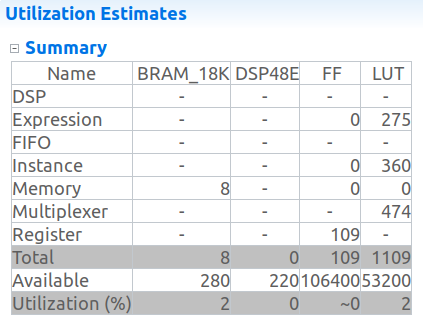
\includegraphics[width=\textwidth]{figs/31a.png}
    \caption{5.1}
    \label{fig:my_label}
\end{subfigure}
\hfill
\begin{subfigure}[b]{0.8\textwidth}
    \centering
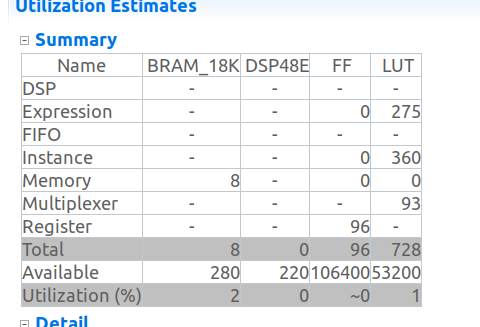
\includegraphics[width=\textwidth]{figs/31b.png}
    \caption{5.2}
    \label{fig:my_label}
\end{subfigure}
\end{figure}

\vspace{15cm}


\section{HLS Timing Report}
\vspace{1cm}
\begin{figure}[h]
\centering
\begin{subfigure}[b]{0.7\textwidth}
    \centering
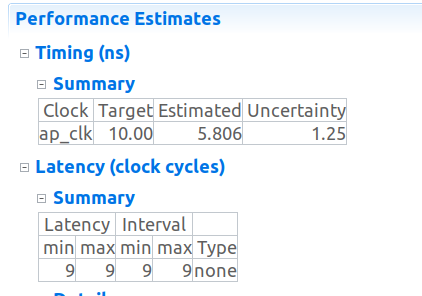
\includegraphics[width=\textwidth]{figs/32a.png}
    \caption{5.1}
    \label{fig:my_label}
\end{subfigure}
\hfill
\begin{subfigure}[b]{0.8\textwidth}
    \centering
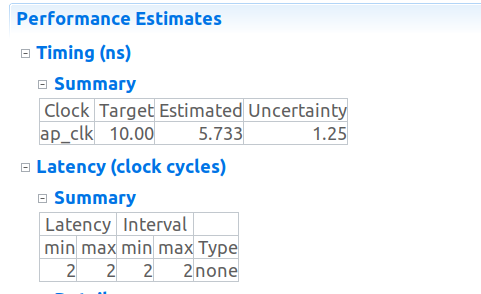
\includegraphics[width=\textwidth]{figs/32b.png}
    \caption{5.2}
    \label{fig:my_label}
\end{subfigure}
\end{figure}

\vspace{15cm}


\section{Interfaces Report}
\vspace{1cm}
\begin{figure}[h]
\centering
\begin{subfigure}[b]{0.5\textwidth}
    \centering
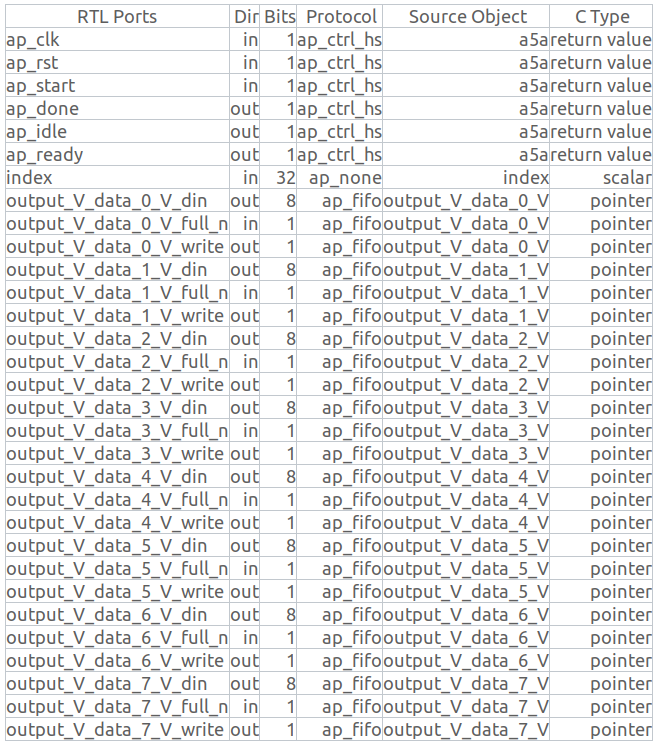
\includegraphics[width=\textwidth]{figs/33a.png}
    \caption{5.1}
    \label{fig:my_label}
\end{subfigure}
\hfill
\begin{subfigure}[b]{0.5\textwidth}
    \centering
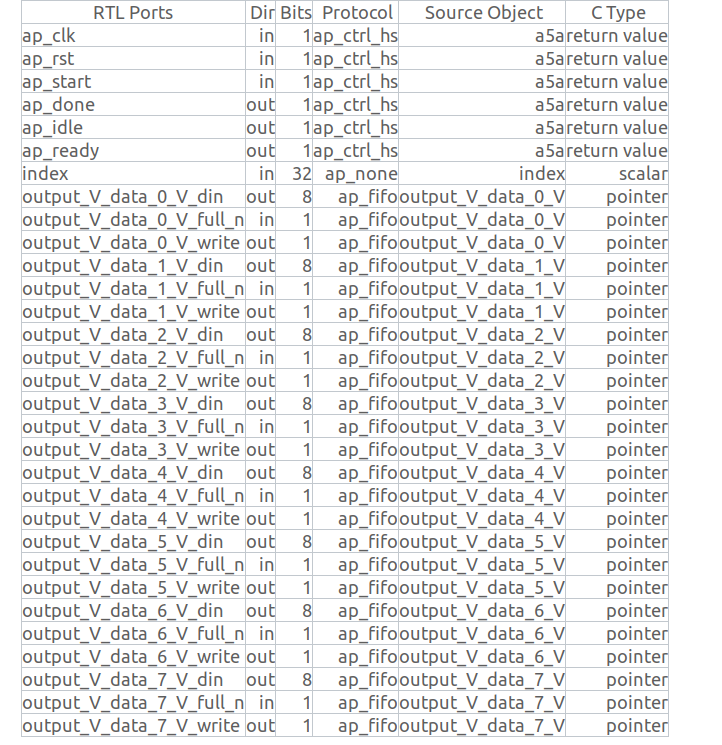
\includegraphics[width=\textwidth]{figs/33b.png}
    \caption{5.2}
    \label{fig:my_label}
\end{subfigure}
\end{figure}
\vspace{15cm}


\section{C/RTL Cosimulation Output}
\vspace{1cm}
\textbf{5.1}
\begin{lstlisting}

Starting C/RTL cosimulation ...
/tools/Xilinx/Vivado/2018.3/bin/vivado_hls /home/sam-admin/git/Training/HLS_Assignments/A5/5.1/codes/Assignmnet5a/solution51a/cosim.tcl
INFO: [HLS 200-10] Running '/tools/Xilinx/Vivado/2018.3/bin/unwrapped/lnx64.o/vivado_hls'
INFO: [HLS 200-10] For user 'sam-admin' on host 'sampaths-lappie' (Linux_x86_64 version 5.19.0-38-generic) on Mon Apr 03 12:39:38 IST 2023
INFO: [HLS 200-10] On os Ubuntu 22.04.2 LTS
INFO: [HLS 200-10] In directory '/home/sam-admin/git/Training/HLS_Assignments/A5/5.1/codes'
INFO: [HLS 200-10] Opening project '/home/sam-admin/git/Training/HLS_Assignments/A5/5.1/codes/Assignmnet5a'.
INFO: [HLS 200-10] Opening solution '/home/sam-admin/git/Training/HLS_Assignments/A5/5.1/codes/Assignmnet5a/solution51a'.
INFO: [SYN 201-201] Setting up clock 'default' with a period of 10ns.
INFO: [HLS 200-10] Setting target device to 'xc7z020clg484-1'
INFO: [COSIM 212-47] Using XSIM for RTL simulation.
INFO: [COSIM 212-14] Instrumenting C test bench ...
   Build using "/tools/Xilinx/Vivado/2018.3/tps/lnx64/gcc-6.2.0/bin/g++"
   Compiling a51a.cpp_pre.cpp.tb.cpp
   Compiling a5a_tb.cpp_pre.cpp.tb.cpp
   Compiling apatb_a5a.cpp
   Generating cosim.tv.exe
INFO: [COSIM 212-302] Starting C TB testing ... 
ALL THE TEST CASES ARE PASSED!
INFO: [COSIM 212-333] Generating C post check test bench ...
INFO: [COSIM 212-12] Generating RTL test bench ...
INFO: [COSIM 212-323] Starting verilog simulation. 
INFO: [COSIM 212-15] Starting XSIM ...
INFO: [XSIM 43-3496] Using init file passed via -initfile option "/tools/Xilinx/Vivado/2018.3/data/xsim/ip/xsim_ip.ini".
Vivado Simulator 2018.3
Copyright 1986-1999, 2001-2018 Xilinx, Inc. All Rights Reserved.
Running: /tools/Xilinx/Vivado/2018.3/bin/unwrapped/lnx64.o/xelab xil_defaultlib.apatb_a5a_top glbl -prj a5a.prj -L smartconnect_v1_0 -L axi_protocol_checker_v1_1_12 -L axi_protocol_checker_v1_1_13 -L axis_protocol_checker_v1_1_11 -L axis_protocol_checker_v1_1_12 -L xil_defaultlib -L unisims_ver -L xpm --initfile /tools/Xilinx/Vivado/2018.3/data/xsim/ip/xsim_ip.ini --lib ieee_proposed=./ieee_proposed -s a5a 
Multi-threading is on. Using 6 slave threads.
WARNING: [XSIM 43-3431] One or more environment variables have been detected which affect the operation of the C compiler. These are typically not set in standard installations and are not tested by Xilinx, however they may be appropriate for your system, so the flow will attempt to continue.  If errors occur, try running xelab with the "-mt off -v 1" switches to see more information from the C compiler. The following environment variables have been detected:
    LIBRARY_PATH
INFO: [VRFC 10-2263] Analyzing SystemVerilog file "/home/sam-admin/git/Training/HLS_Assignments/A5/5.1/codes/Assignmnet5a/solution51a/sim/verilog/glbl.v" into library work
INFO: [VRFC 10-311] analyzing module glbl
INFO: [VRFC 10-2263] Analyzing SystemVerilog file "/home/sam-admin/git/Training/HLS_Assignments/A5/5.1/codes/Assignmnet5a/solution51a/sim/verilog/AESL_autofifo_output_V_data_6_V.v" into library xil_defaultlib
INFO: [VRFC 10-311] analyzing module AESL_autofifo_output_V_data_6_V
INFO: [VRFC 10-2263] Analyzing SystemVerilog file "/home/sam-admin/git/Training/HLS_Assignments/A5/5.1/codes/Assignmnet5a/solution51a/sim/verilog/AESL_autofifo_output_V_data_3_V.v" into library xil_defaultlib
INFO: [VRFC 10-311] analyzing module AESL_autofifo_output_V_data_3_V
INFO: [VRFC 10-2263] Analyzing SystemVerilog file "/home/sam-admin/git/Training/HLS_Assignments/A5/5.1/codes/Assignmnet5a/solution51a/sim/verilog/a5a_bram_4.v" into library xil_defaultlib
INFO: [VRFC 10-311] analyzing module a5a_bram_4_rom
INFO: [VRFC 10-311] analyzing module a5a_bram_4
INFO: [VRFC 10-2263] Analyzing SystemVerilog file "/home/sam-admin/git/Training/HLS_Assignments/A5/5.1/codes/Assignmnet5a/solution51a/sim/verilog/AESL_autofifo_output_V_data_7_V.v" into library xil_defaultlib
INFO: [VRFC 10-311] analyzing module AESL_autofifo_output_V_data_7_V
INFO: [VRFC 10-2263] Analyzing SystemVerilog file "/home/sam-admin/git/Training/HLS_Assignments/A5/5.1/codes/Assignmnet5a/solution51a/sim/verilog/a5a_bram_7.v" into library xil_defaultlib
INFO: [VRFC 10-311] analyzing module a5a_bram_7_rom
INFO: [VRFC 10-311] analyzing module a5a_bram_7
INFO: [VRFC 10-2263] Analyzing SystemVerilog file "/home/sam-admin/git/Training/HLS_Assignments/A5/5.1/codes/Assignmnet5a/solution51a/sim/verilog/a5a_bram_0.v" into library xil_defaultlib
INFO: [VRFC 10-311] analyzing module a5a_bram_0_rom
INFO: [VRFC 10-311] analyzing module a5a_bram_0
INFO: [VRFC 10-2263] Analyzing SystemVerilog file "/home/sam-admin/git/Training/HLS_Assignments/A5/5.1/codes/Assignmnet5a/solution51a/sim/verilog/a5a_bram_6.v" into library xil_defaultlib
INFO: [VRFC 10-311] analyzing module a5a_bram_6_rom
INFO: [VRFC 10-311] analyzing module a5a_bram_6
INFO: [VRFC 10-2263] Analyzing SystemVerilog file "/home/sam-admin/git/Training/HLS_Assignments/A5/5.1/codes/Assignmnet5a/solution51a/sim/verilog/AESL_autofifo_output_V_data_0_V.v" into library xil_defaultlib
INFO: [VRFC 10-311] analyzing module AESL_autofifo_output_V_data_0_V
INFO: [VRFC 10-2263] Analyzing SystemVerilog file "/home/sam-admin/git/Training/HLS_Assignments/A5/5.1/codes/Assignmnet5a/solution51a/sim/verilog/AESL_autofifo_output_V_data_2_V.v" into library xil_defaultlib
INFO: [VRFC 10-311] analyzing module AESL_autofifo_output_V_data_2_V
INFO: [VRFC 10-2263] Analyzing SystemVerilog file "/home/sam-admin/git/Training/HLS_Assignments/A5/5.1/codes/Assignmnet5a/solution51a/sim/verilog/a5a_bram_2.v" into library xil_defaultlib
INFO: [VRFC 10-311] analyzing module a5a_bram_2_rom
INFO: [VRFC 10-311] analyzing module a5a_bram_2
INFO: [VRFC 10-2263] Analyzing SystemVerilog file "/home/sam-admin/git/Training/HLS_Assignments/A5/5.1/codes/Assignmnet5a/solution51a/sim/verilog/a5a_bram_5.v" into library xil_defaultlib
INFO: [VRFC 10-311] analyzing module a5a_bram_5_rom
INFO: [VRFC 10-311] analyzing module a5a_bram_5
INFO: [VRFC 10-2263] Analyzing SystemVerilog file "/home/sam-admin/git/Training/HLS_Assignments/A5/5.1/codes/Assignmnet5a/solution51a/sim/verilog/a5a_mux_832_8_1_1.v" into library xil_defaultlib
INFO: [VRFC 10-311] analyzing module a5a_mux_832_8_1_1
INFO: [VRFC 10-2263] Analyzing SystemVerilog file "/home/sam-admin/git/Training/HLS_Assignments/A5/5.1/codes/Assignmnet5a/solution51a/sim/verilog/a5a_bram_3.v" into library xil_defaultlib
INFO: [VRFC 10-311] analyzing module a5a_bram_3_rom
INFO: [VRFC 10-311] analyzing module a5a_bram_3
INFO: [VRFC 10-2263] Analyzing SystemVerilog file "/home/sam-admin/git/Training/HLS_Assignments/A5/5.1/codes/Assignmnet5a/solution51a/sim/verilog/a5a.v" into library xil_defaultlib
INFO: [VRFC 10-311] analyzing module a5a
INFO: [VRFC 10-2263] Analyzing SystemVerilog file "/home/sam-admin/git/Training/HLS_Assignments/A5/5.1/codes/Assignmnet5a/solution51a/sim/verilog/AESL_autofifo_output_V_data_4_V.v" into library xil_defaultlib
INFO: [VRFC 10-311] analyzing module AESL_autofifo_output_V_data_4_V
INFO: [VRFC 10-2263] Analyzing SystemVerilog file "/home/sam-admin/git/Training/HLS_Assignments/A5/5.1/codes/Assignmnet5a/solution51a/sim/verilog/a5a.autotb.v" into library xil_defaultlib
INFO: [VRFC 10-311] analyzing module apatb_a5a_top
INFO: [VRFC 10-2263] Analyzing SystemVerilog file "/home/sam-admin/git/Training/HLS_Assignments/A5/5.1/codes/Assignmnet5a/solution51a/sim/verilog/AESL_autofifo_output_V_data_5_V.v" into library xil_defaultlib
INFO: [VRFC 10-311] analyzing module AESL_autofifo_output_V_data_5_V
INFO: [VRFC 10-2263] Analyzing SystemVerilog file "/home/sam-admin/git/Training/HLS_Assignments/A5/5.1/codes/Assignmnet5a/solution51a/sim/verilog/AESL_autofifo_output_V_data_1_V.v" into library xil_defaultlib
INFO: [VRFC 10-311] analyzing module AESL_autofifo_output_V_data_1_V
INFO: [VRFC 10-2263] Analyzing SystemVerilog file "/home/sam-admin/git/Training/HLS_Assignments/A5/5.1/codes/Assignmnet5a/solution51a/sim/verilog/a5a_bram_1.v" into library xil_defaultlib
INFO: [VRFC 10-311] analyzing module a5a_bram_1_rom
INFO: [VRFC 10-311] analyzing module a5a_bram_1
Starting static elaboration
Completed static elaboration
Starting simulation data flow analysis
Completed simulation data flow analysis
Time Resolution for simulation is 1ps
Compiling module xil_defaultlib.a5a_bram_0_rom
Compiling module xil_defaultlib.a5a_bram_0(DataWidth=6,AddressRa...
Compiling module xil_defaultlib.a5a_bram_1_rom
Compiling module xil_defaultlib.a5a_bram_1(DataWidth=6,AddressRa...
Compiling module xil_defaultlib.a5a_bram_2_rom
Compiling module xil_defaultlib.a5a_bram_2(DataWidth=6,AddressRa...
Compiling module xil_defaultlib.a5a_bram_3_rom
Compiling module xil_defaultlib.a5a_bram_3(DataWidth=6,AddressRa...
Compiling module xil_defaultlib.a5a_bram_4_rom
Compiling module xil_defaultlib.a5a_bram_4(DataWidth=6,AddressRa...
Compiling module xil_defaultlib.a5a_bram_5_rom
Compiling module xil_defaultlib.a5a_bram_5(DataWidth=6,AddressRa...
Compiling module xil_defaultlib.a5a_bram_6_rom
Compiling module xil_defaultlib.a5a_bram_6(DataWidth=6,AddressRa...
Compiling module xil_defaultlib.a5a_bram_7_rom
Compiling module xil_defaultlib.a5a_bram_7(DataWidth=6,AddressRa...
Compiling module xil_defaultlib.a5a_mux_832_8_1_1(ID=1,din0_WIDT...
Compiling module xil_defaultlib.a5a
Compiling module xil_defaultlib.AESL_autofifo_output_V_data_0_V
Compiling module xil_defaultlib.AESL_autofifo_output_V_data_1_V
Compiling module xil_defaultlib.AESL_autofifo_output_V_data_2_V
Compiling module xil_defaultlib.AESL_autofifo_output_V_data_3_V
Compiling module xil_defaultlib.AESL_autofifo_output_V_data_4_V
Compiling module xil_defaultlib.AESL_autofifo_output_V_data_5_V
Compiling module xil_defaultlib.AESL_autofifo_output_V_data_6_V
Compiling module xil_defaultlib.AESL_autofifo_output_V_data_7_V
Compiling module xil_defaultlib.apatb_a5a_top
Compiling module work.glbl
Built simulation snapshot a5a


****** Webtalk v2018.3 (64-bit)
  **** SW Build 2405991 on Thu Dec  6 23:36:41 MST 2018
  **** IP Build 2404404 on Fri Dec  7 01:43:56 MST 2018
    ** Copyright 1986-2018 Xilinx, Inc. All Rights Reserved.


source /home/sam-admin/git/Training/HLS_Assignments/A5/5.1/codes/Assignmnet5a/solution51a/sim/verilog/xsim.dir/a5a/webtalk/xsim_webtalk.tcl -notrace
INFO: [Common 17-206] Exiting Webtalk at Mon Apr  3 12:40:39 2023...


****** xsim v2018.3 (64-bit)
  **** SW Build 2405991 on Thu Dec  6 23:36:41 MST 2018
  **** IP Build 2404404 on Fri Dec  7 01:43:56 MST 2018
    ** Copyright 1986-2018 Xilinx, Inc. All Rights Reserved.


source xsim.dir/a5a/xsim_script.tcl
# xsim {a5a} -autoloadwcfg -tclbatch {a5a.tcl}
Vivado Simulator 2018.3
Time resolution is 1 ps
source a5a.tcl
## run all
////////////////////////////////////////////////////////////////////////////////////
// Inter-Transaction Progress: Completed Transaction / Total Transaction
// Intra-Transaction Progress: Measured Latency / Latency Estimation * 100%
//
// RTL Simulation : "Inter-Transaction Progress" ["Intra-Transaction Progress"] @ "Simulation Time"
////////////////////////////////////////////////////////////////////////////////////
// RTL Simulation : 0 / 8 [0.00%] @ "125000"
// RTL Simulation : 1 / 8 [100.00%] @ "235000"
// RTL Simulation : 2 / 8 [100.00%] @ "335000"
// RTL Simulation : 3 / 8 [100.00%] @ "435000"
// RTL Simulation : 4 / 8 [100.00%] @ "535000"
// RTL Simulation : 5 / 8 [100.00%] @ "635000"
// RTL Simulation : 6 / 8 [100.00%] @ "735000"
// RTL Simulation : 7 / 8 [100.00%] @ "835000"
// RTL Simulation : 8 / 8 [100.00%] @ "935000"
////////////////////////////////////////////////////////////////////////////////////
$finish called at time : 975 ns : File "/home/sam-admin/git/Training/HLS_Assignments/A5/5.1/codes/Assignmnet5a/solution51a/sim/verilog/a5a.autotb.v" Line 671
## quit
INFO: [Common 17-206] Exiting xsim at Mon Apr  3 12:40:57 2023...
INFO: [COSIM 212-316] Starting C post checking ...
ALL THE TEST CASES ARE PASSED!
INFO: [COSIM 212-1000] *** C/RTL co-simulation finished: PASS ***
Finished C/RTL cosimulation.



\end{lstlisting}
\vspace{3cm}
\textbf{5.2}
\vspace{1cm}
\begin{lstlisting}
Starting C/RTL cosimulation ...
/tools/Xilinx/Vivado/2018.3/bin/vivado_hls /home/sam-admin/git/Training/HLS_Assignments/A5/5.1/codes/Assignmnet5a/solution52a/cosim.tcl
INFO: [HLS 200-10] Running '/tools/Xilinx/Vivado/2018.3/bin/unwrapped/lnx64.o/vivado_hls'
INFO: [HLS 200-10] For user 'sam-admin' on host 'sampaths-lappie' (Linux_x86_64 version 5.19.0-38-generic) on Mon Apr 03 13:46:38 IST 2023
INFO: [HLS 200-10] On os Ubuntu 22.04.2 LTS
INFO: [HLS 200-10] In directory '/home/sam-admin/git/Training/HLS_Assignments/A5/5.1/codes'
INFO: [HLS 200-10] Opening project '/home/sam-admin/git/Training/HLS_Assignments/A5/5.1/codes/Assignmnet5a'.
INFO: [HLS 200-10] Opening solution '/home/sam-admin/git/Training/HLS_Assignments/A5/5.1/codes/Assignmnet5a/solution52a'.
INFO: [SYN 201-201] Setting up clock 'default' with a period of 10ns.
INFO: [HLS 200-10] Setting target device to 'xc7z020clg484-1'
INFO: [COSIM 212-47] Using XSIM for RTL simulation.
INFO: [COSIM 212-14] Instrumenting C test bench ...
   Build using "/tools/Xilinx/Vivado/2018.3/tps/lnx64/gcc-6.2.0/bin/g++"
   Compiling a51a.cpp_pre.cpp.tb.cpp
   Compiling a5a_tb.cpp_pre.cpp.tb.cpp
   Compiling apatb_a5a.cpp
   Generating cosim.tv.exe
INFO: [COSIM 212-302] Starting C TB testing ... 
ALL THE TEST CASES ARE PASSED!
INFO: [COSIM 212-333] Generating C post check test bench ...
INFO: [COSIM 212-12] Generating RTL test bench ...
INFO: [COSIM 212-323] Starting verilog simulation. 
INFO: [COSIM 212-15] Starting XSIM ...
INFO: [XSIM 43-3496] Using init file passed via -initfile option "/tools/Xilinx/Vivado/2018.3/data/xsim/ip/xsim_ip.ini".
Vivado Simulator 2018.3
Copyright 1986-1999, 2001-2018 Xilinx, Inc. All Rights Reserved.
Running: /tools/Xilinx/Vivado/2018.3/bin/unwrapped/lnx64.o/xelab xil_defaultlib.apatb_a5a_top glbl -prj a5a.prj -L smartconnect_v1_0 -L axi_protocol_checker_v1_1_12 -L axi_protocol_checker_v1_1_13 -L axis_protocol_checker_v1_1_11 -L axis_protocol_checker_v1_1_12 -L xil_defaultlib -L unisims_ver -L xpm --initfile /tools/Xilinx/Vivado/2018.3/data/xsim/ip/xsim_ip.ini --lib ieee_proposed=./ieee_proposed -s a5a 
Multi-threading is on. Using 6 slave threads.
WARNING: [XSIM 43-3431] One or more environment variables have been detected which affect the operation of the C compiler. These are typically not set in standard installations and are not tested by Xilinx, however they may be appropriate for your system, so the flow will attempt to continue.  If errors occur, try running xelab with the "-mt off -v 1" switches to see more information from the C compiler. The following environment variables have been detected:
    LIBRARY_PATH
INFO: [VRFC 10-2263] Analyzing SystemVerilog file "/home/sam-admin/git/Training/HLS_Assignments/A5/5.1/codes/Assignmnet5a/solution52a/sim/verilog/glbl.v" into library work
INFO: [VRFC 10-311] analyzing module glbl
INFO: [VRFC 10-2263] Analyzing SystemVerilog file "/home/sam-admin/git/Training/HLS_Assignments/A5/5.1/codes/Assignmnet5a/solution52a/sim/verilog/AESL_autofifo_output_V_data_6_V.v" into library xil_defaultlib
INFO: [VRFC 10-311] analyzing module AESL_autofifo_output_V_data_6_V
INFO: [VRFC 10-2263] Analyzing SystemVerilog file "/home/sam-admin/git/Training/HLS_Assignments/A5/5.1/codes/Assignmnet5a/solution52a/sim/verilog/AESL_autofifo_output_V_data_3_V.v" into library xil_defaultlib
INFO: [VRFC 10-311] analyzing module AESL_autofifo_output_V_data_3_V
INFO: [VRFC 10-2263] Analyzing SystemVerilog file "/home/sam-admin/git/Training/HLS_Assignments/A5/5.1/codes/Assignmnet5a/solution52a/sim/verilog/a5a_bram_4.v" into library xil_defaultlib
INFO: [VRFC 10-311] analyzing module a5a_bram_4_rom
INFO: [VRFC 10-311] analyzing module a5a_bram_4
INFO: [VRFC 10-2263] Analyzing SystemVerilog file "/home/sam-admin/git/Training/HLS_Assignments/A5/5.1/codes/Assignmnet5a/solution52a/sim/verilog/AESL_autofifo_output_V_data_7_V.v" into library xil_defaultlib
INFO: [VRFC 10-311] analyzing module AESL_autofifo_output_V_data_7_V
INFO: [VRFC 10-2263] Analyzing SystemVerilog file "/home/sam-admin/git/Training/HLS_Assignments/A5/5.1/codes/Assignmnet5a/solution52a/sim/verilog/a5a_bram_0.v" into library xil_defaultlib
INFO: [VRFC 10-311] analyzing module a5a_bram_0_rom
INFO: [VRFC 10-311] analyzing module a5a_bram_0
INFO: [VRFC 10-2263] Analyzing SystemVerilog file "/home/sam-admin/git/Training/HLS_Assignments/A5/5.1/codes/Assignmnet5a/solution52a/sim/verilog/AESL_autofifo_output_V_data_0_V.v" into library xil_defaultlib
INFO: [VRFC 10-311] analyzing module AESL_autofifo_output_V_data_0_V
INFO: [VRFC 10-2263] Analyzing SystemVerilog file "/home/sam-admin/git/Training/HLS_Assignments/A5/5.1/codes/Assignmnet5a/solution52a/sim/verilog/AESL_autofifo_output_V_data_2_V.v" into library xil_defaultlib
INFO: [VRFC 10-311] analyzing module AESL_autofifo_output_V_data_2_V
INFO: [VRFC 10-2263] Analyzing SystemVerilog file "/home/sam-admin/git/Training/HLS_Assignments/A5/5.1/codes/Assignmnet5a/solution52a/sim/verilog/a5a_bram_2.v" into library xil_defaultlib
INFO: [VRFC 10-311] analyzing module a5a_bram_2_rom
INFO: [VRFC 10-311] analyzing module a5a_bram_2
INFO: [VRFC 10-2263] Analyzing SystemVerilog file "/home/sam-admin/git/Training/HLS_Assignments/A5/5.1/codes/Assignmnet5a/solution52a/sim/verilog/a5a_bram_5.v" into library xil_defaultlib
INFO: [VRFC 10-311] analyzing module a5a_bram_5_rom
INFO: [VRFC 10-311] analyzing module a5a_bram_5
INFO: [VRFC 10-2263] Analyzing SystemVerilog file "/home/sam-admin/git/Training/HLS_Assignments/A5/5.1/codes/Assignmnet5a/solution52a/sim/verilog/a5a_mux_832_8_1_1.v" into library xil_defaultlib
INFO: [VRFC 10-311] analyzing module a5a_mux_832_8_1_1
INFO: [VRFC 10-2263] Analyzing SystemVerilog file "/home/sam-admin/git/Training/HLS_Assignments/A5/5.1/codes/Assignmnet5a/solution52a/sim/verilog/a5a.v" into library xil_defaultlib
INFO: [VRFC 10-311] analyzing module a5a
INFO: [VRFC 10-2263] Analyzing SystemVerilog file "/home/sam-admin/git/Training/HLS_Assignments/A5/5.1/codes/Assignmnet5a/solution52a/sim/verilog/AESL_autofifo_output_V_data_4_V.v" into library xil_defaultlib
INFO: [VRFC 10-311] analyzing module AESL_autofifo_output_V_data_4_V
INFO: [VRFC 10-2263] Analyzing SystemVerilog file "/home/sam-admin/git/Training/HLS_Assignments/A5/5.1/codes/Assignmnet5a/solution52a/sim/verilog/a5a.autotb.v" into library xil_defaultlib
INFO: [VRFC 10-311] analyzing module apatb_a5a_top
INFO: [VRFC 10-2263] Analyzing SystemVerilog file "/home/sam-admin/git/Training/HLS_Assignments/A5/5.1/codes/Assignmnet5a/solution52a/sim/verilog/AESL_autofifo_output_V_data_5_V.v" into library xil_defaultlib
INFO: [VRFC 10-311] analyzing module AESL_autofifo_output_V_data_5_V
INFO: [VRFC 10-2263] Analyzing SystemVerilog file "/home/sam-admin/git/Training/HLS_Assignments/A5/5.1/codes/Assignmnet5a/solution52a/sim/verilog/AESL_autofifo_output_V_data_1_V.v" into library xil_defaultlib
INFO: [VRFC 10-311] analyzing module AESL_autofifo_output_V_data_1_V
INFO: [VRFC 10-2263] Analyzing SystemVerilog file "/home/sam-admin/git/Training/HLS_Assignments/A5/5.1/codes/Assignmnet5a/solution52a/sim/verilog/a5a_bram_1.v" into library xil_defaultlib
INFO: [VRFC 10-311] analyzing module a5a_bram_1_rom
INFO: [VRFC 10-311] analyzing module a5a_bram_1
Starting static elaboration
Completed static elaboration
Starting simulation data flow analysis
Completed simulation data flow analysis
Time Resolution for simulation is 1ps
Compiling module xil_defaultlib.a5a_bram_0_rom
Compiling module xil_defaultlib.a5a_bram_0(DataWidth=3,AddressRa...
Compiling module xil_defaultlib.a5a_bram_1_rom
Compiling module xil_defaultlib.a5a_bram_1(DataWidth=4,AddressRa...
Compiling module xil_defaultlib.a5a_bram_2_rom
Compiling module xil_defaultlib.a5a_bram_2(DataWidth=5,AddressRa...
Compiling module xil_defaultlib.a5a_bram_4_rom
Compiling module xil_defaultlib.a5a_bram_4(DataWidth=6,AddressRa...
Compiling module xil_defaultlib.a5a_bram_5_rom
Compiling module xil_defaultlib.a5a_bram_5(DataWidth=6,AddressRa...
Compiling module xil_defaultlib.a5a_mux_832_8_1_1(ID=1,din0_WIDT...
Compiling module xil_defaultlib.a5a
Compiling module xil_defaultlib.AESL_autofifo_output_V_data_0_V
Compiling module xil_defaultlib.AESL_autofifo_output_V_data_1_V
Compiling module xil_defaultlib.AESL_autofifo_output_V_data_2_V
Compiling module xil_defaultlib.AESL_autofifo_output_V_data_3_V
Compiling module xil_defaultlib.AESL_autofifo_output_V_data_4_V
Compiling module xil_defaultlib.AESL_autofifo_output_V_data_5_V
Compiling module xil_defaultlib.AESL_autofifo_output_V_data_6_V
Compiling module xil_defaultlib.AESL_autofifo_output_V_data_7_V
Compiling module xil_defaultlib.apatb_a5a_top
Compiling module work.glbl
Built simulation snapshot a5a


****** Webtalk v2018.3 (64-bit)
  **** SW Build 2405991 on Thu Dec  6 23:36:41 MST 2018
  **** IP Build 2404404 on Fri Dec  7 01:43:56 MST 2018
    ** Copyright 1986-2018 Xilinx, Inc. All Rights Reserved.


source /home/sam-admin/git/Training/HLS_Assignments/A5/5.1/codes/Assignmnet5a/solution52a/sim/verilog/xsim.dir/a5a/webtalk/xsim_webtalk.tcl -notrace
INFO: [Common 17-206] Exiting Webtalk at Mon Apr  3 13:47:26 2023...


****** xsim v2018.3 (64-bit)
  **** SW Build 2405991 on Thu Dec  6 23:36:41 MST 2018
  **** IP Build 2404404 on Fri Dec  7 01:43:56 MST 2018
    ** Copyright 1986-2018 Xilinx, Inc. All Rights Reserved.


source xsim.dir/a5a/xsim_script.tcl
# xsim {a5a} -autoloadwcfg -tclbatch {a5a.tcl}
Vivado Simulator 2018.3
Time resolution is 1 ps
source a5a.tcl
## run all
////////////////////////////////////////////////////////////////////////////////////
// Inter-Transaction Progress: Completed Transaction / Total Transaction
// Intra-Transaction Progress: Measured Latency / Latency Estimation * 100%
//
// RTL Simulation : "Inter-Transaction Progress" ["Intra-Transaction Progress"] @ "Simulation Time"
////////////////////////////////////////////////////////////////////////////////////
// RTL Simulation : 0 / 8 [0.00%] @ "125000"
// RTL Simulation : 1 / 8 [100.00%] @ "165000"
// RTL Simulation : 2 / 8 [100.00%] @ "195000"
// RTL Simulation : 3 / 8 [100.00%] @ "225000"
// RTL Simulation : 4 / 8 [100.00%] @ "255000"
// RTL Simulation : 5 / 8 [100.00%] @ "285000"
// RTL Simulation : 6 / 8 [100.00%] @ "315000"
// RTL Simulation : 7 / 8 [100.00%] @ "345000"
// RTL Simulation : 8 / 8 [100.00%] @ "375000"
////////////////////////////////////////////////////////////////////////////////////
$finish called at time : 415 ns : File "/home/sam-admin/git/Training/HLS_Assignments/A5/5.1/codes/Assignmnet5a/solution52a/sim/verilog/a5a.autotb.v" Line 671
## quit
INFO: [Common 17-206] Exiting xsim at Mon Apr  3 13:47:44 2023...
INFO: [COSIM 212-316] Starting C post checking ...
ALL THE TEST CASES ARE PASSED!
INFO: [COSIM 212-1000] *** C/RTL co-simulation finished: PASS ***
Finished C/RTL cosimulation.


\end{lstlisting}
\vspace{3cm}


\section{C/RTL Cosimulation Report}
\vspace{1cm}
\begin{figure}[h]
\centering
\begin{subfigure}[b]{0.8\textwidth}
    \centering
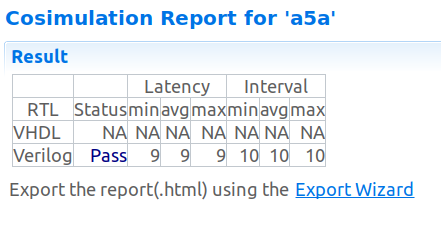
\includegraphics[width=\textwidth]{figs/34a.png}
    \caption{5.1}
    \label{fig:my_label}
\end{subfigure}
\hfill
\begin{subfigure}[b]{0.8\textwidth}
    \centering
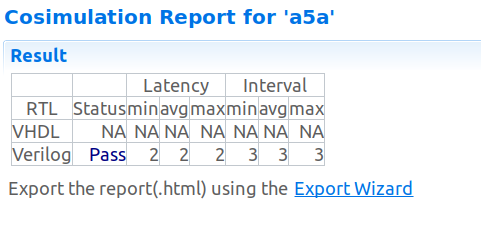
\includegraphics[width=\textwidth]{figs/34b.png}
    \caption{5.2}
    \label{fig:my_label}
\end{subfigure}
\end{figure}

\vspace{5cm}


\end{document}
